\chapter{Ecuaciones Diferenciales en Física}

En física, es muy común que diversas situaciones sean modeladas no por ecuaciones que únicamente contengan potencias (enteras o semienteras) de alguna variable física, sino que incluyan derivadas de estas.

En sus cursos de Mecánica y de Ecuaciones Diferenciales, probablemente se familiarizaron con los casos del Oscilador Armónico y del Oscilador amortiguado, que son descritos por las ecuaciones \eqref{eq:mas} y \eqref{eq:amortiguado}, respectivamente.

\begin{gather}
    \frac{d^2x}{dt^2} = - \omega^2 x \ , \label{eq:mas} \\
    \frac{d^2x}{dt^2} + 2\gamma \frac{dx}{dt} + \omega^2_0 x = 0 \ . \label{eq:amortiguado}
\end{gather}

Ambas ecuaciones consisten en ecuaciones diferenciales \emph{ordinarias}, debido a que la función a derivar, $x(t)$, depende de una única variable,por lo cual todas las derivadas en ella son totales.

Sin embargo, muchas otras situaciones físicas no pueden ser descritas únicamente en términos de funciones de una sola variable, incluso cuando dicha función solo dependa de la posición. Por ejemplo, podríamos querer describir el potencial eléctrico de una distribución esférica de cargas, cuya densidad dependa de nuestra posición tanto respecto al centro de la esfera (variable $r$), así como también respecto al ángulo que forma con respecto de su polo norte (variable $\theta$), de modo que este potencial será una función tanto de $r$ como de $\theta$. Este tipo de sistemas serán descritos por ecuaciones diferenciales \emph{parciales} (EDPs).

Hasta el día de hoy, el desarrollo de métodos para resolver EDPs es un área de investigación activa en matemáticas, por lo que en este curso nos limitaremos a algunos de los métodos más tradicionales y que son la base para la descripción de la física de los siglos XVIII y XIX, como lo son la mecánica hamiltoniana, la teoría clásica de campos o la electrodinámica clásica.

\section{Algunas ecuaciones básicas}

A continuación listamos algunos ejemplos de EDPs \emph{lineales} en la función incógnita $\psi$, y de, a lo más, \emph{segundo orden}. Algunos puntos que mencionar antes de entrar en ellas, es que siempre que veamos una derivada respecto al tiempo, esto quiere decir que la función incógnita \emph{tendrá una evolución temporal}. 

También cabe mencionar que no todos los sistemas físicos pueden ser descritos por ecuaciones ``bien portadas'' como las que listaremos a continuación, ya que por ejemplo, en fenómenos que involucren turbulencias, como la física de plasmas o la física atmosférica, las ecuaciones son no lineales, lo que complica la posibilidad de resolverlas de forma analítica, y se encuentran fuera del alcance de este curso.

\subsection*{Ecuación de Laplace}

Esta corresponde a la expresión
\begin{equation}
    \nabla^2 \psi = 0 \ ,
\end{equation}
la que surge en el estudio de diferentes sistemas físicos, como por ejemplo:
\begin{itemize}
    \item el \textbf{potencial electrostático} en una región sin cargas. 
    \item un \textbf{fluido irrotacional incompresible} en un movimiento estacionario, cuyo campo de velocidades es descrito como $\vec{v} = -\nabla \psi$.
    \item el \textbf{potencial gravitatorio}.
    \item una \textbf{distribución de temperatura estacionaria}, donde en este caso $\psi = T(x,t)$ corresponde al campo de temperaturas de un material.
\end{itemize}

\subsection*{Ecuación de Poisson}

Esta corresponde, por llamarlo de una manera, a la generalización de la ecuación de Laplace para cualquier sistema con una función \emph{fuente} $f$ conocida. Es dada por la expresión
\begin{equation}
    \nabla^2\psi = f(\vec{x}) \ .
\end{equation}

Esta corresponde a una ecuación \emph{inhomogénea}, cuyas soluciones generales pueden escribirse como $\psi = \psi_h + \psi_p$, donde el primer término corresponde a la solución de la \emph{ecuación homogénea} donde $f(x) = 0$, que en este caso corresponde a la ecuación de Laplace, y el segundo término es una \emph{solución particular} de la ecuación de Poisson.

Esta puede surgir en situaciones similares a la ecuación de Laplace, pero en las cuales existen \emph{fuentes} para los respectivos campos. Por ejemplo, para el caso electrostático, puede existir una fuente con densidad de carga $\rho(\vec{x})$, de modo que la ecuación que describe el potencial eléctrico en dicha región será
\begin{equation}
    \nabla^2 \phi = - \frac{\rho(\vec{x})}{\varepsilon_0} \ .
\end{equation}

\subsection*{Ecuación de Helmholtz}

Es una ecuación que surge al aplicar el método de separación de variables a una ecuación de onda (siendo ambos términos explicados más abajo), de modo que es una especie de \emph{ecuación de onda independiente del tiempo}, o en otros contextos, una \emph{ecuación de difusión independiente del tiempo}. Se escribe como
\begin{equation}
    \nabla^2 \psi \pm k^2 \psi = 0 \ .
\end{equation}

Esta ecuación aparece en el estudio de diversas áreas, como la radiación electromagnética, la sismología, la acústica o el estudio de membranas (ondas elásticas en medios continuos).



\subsection*{Ecuación de difusión de calor dependiente del tiempo}

Su nombre es autodescriptivo. Las series de Fourier surgen como un método para resolver esta ecuación en el siglo XIX.

\begin{equation}
    \nabla^2 \psi - \frac{1}{\alpha} \frac{\partial \psi}{\partial t} = 0 \ ,
\end{equation}
donde $\alpha$ corresponde al coeficiente de difusión térmica.

\subsection*{Ecuación de onda dependiente del tiempo}

Describe la propagación de una onda $\psi$ tanto espacial como temporalmente. Suele escribirse como
\begin{equation}
    \nabla^2 \psi - \frac{1}{v^2}\frac{\partial^2 \psi}{\partial t^2} = 0 \ ,
\end{equation}
o bien, definiendo el operador \emph{d'Alembertiano} (comúnmente pronunciado como \emph{box}) como $\square \equiv \frac{1}{v^2} \frac{\partial^2}{\partial t^2} - \nabla^2$,
\begin{equation}
    \square \psi = 0 \ .
\end{equation}

\subsection*{Ecuación de Klein-Gordon}

Corresponde a una generalización de la ecuación de onda para trabajar con sistemas cuánticos relativistas, como es el trabajo de la física de partículas. Esta incorpora las constantes $\hbar$ y $c$, que corresponden respectivamente a la constante de Planck reducida, y que es una de las constantes que nos indicará que estamos trabajando con un sistema cuántico; y a la velocidad de la luz, que nos indica que trabajamos con un sistema relativista. Es dada por
\begin{equation}
    \square \psi - \frac{m^2c^2}{\hbar^2}\psi = 0 \ .
\end{equation}


\subsection*{Ecuación de Schrödinger dependiente del tiempo}
Esta corresponde al límite no relativista de la ecuación de Klein-Gordon (es decir, cuando $c \sim \infty$) y es la que describe la evolución de un sistema en Mecánica Cuántica. Es dada por
\begin{equation}
    i \hbar \frac{\partial \psi}{\partial t}(x,t) = \left( -\frac{\hbar^2}{2m} \nabla^2 + V(x) \right) \psi(x,t) = \hat{H}\psi(x,t) \ .
\end{equation}

% \subsection{Ecuaciones de Maxwell}

% Hasta ahora, todas las ecuaciones listadas anteriormente son lineales en la función $\psi$, que corresponde a nuestra incógnita. A su vez, todas ellas son ecuaciones de segundo orden.

% Las ecuaciones de Maxwell, que corresponden a las ecuaciones diferenciales que describen l, no cumplen ninguna de las condiciones anteriores.


\section{Condiciones de borde}

Para una EDP dada, las soluciones dependerán del dominio $\Omega$ en que queramos trabajar. Por ejemplo, un potencial electrostático en el vacío debe cumplir la ecuación de Laplace, pero será distinto en una esfera de radio $r$ que en un cilindro de largo $\ell$ y radio $\rho$. 

Por ello, debemos entregar información adicional a nuestro problema para poder resolver el problema. Esta información suele denominarse \textbf{condiciones de borde}, \textbf{de frontera} o \textbf{de contorno}, ya que tradicionalmente dan información del comportamiento de la función en los límites o bordes $\partial \Omega$ del sistema (véase figura \ref{fig:condicionesdeborde}).

\begin{figure}[htb]
    \centering
    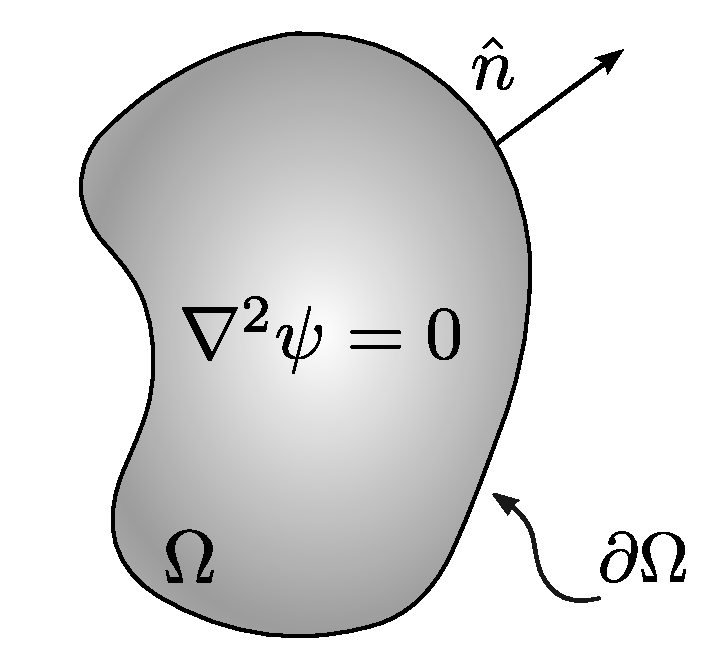
\includegraphics[width = 6cm]{Figuras/Condiciones-Borde.pdf}
    \caption{Dominio $\Omega$ de la ecuación de Laplace con borde $\partial \Omega$ y vector normal $\hat{n}$.}
    \label{fig:condicionesdeborde}
\end{figure}

Puede ser útil clasificar las condiciones de contorno en tres tipos, aplicables a EDPs de segundo orden.

\begin{itemize}
    \item Tenemos condiciones de tipo \textbf{Dirichlet} cuando nos dan información del comportamiento \emph{de la función} $\psi$ en la frontera $\partial \Omega$ de la región en que trabajamos.
    \item Tenemos condiciones de tipo \textbf{Neumann} cuando tenemos información de la \emph{derivada normal de la función}, es decir $\partial \psi/\partial n := \hat{n} \cdot \nabla \psi$, en la frontera $\partial \Omega$.
    \item Tenemos condiciones de tipo \textbf{Cauchy} cuando tenemos a la vez condiciones de tipo Dirichlet y de tipo Neumann.
\end{itemize} 

¿Cómo sabemos qué tipo de condición de borde es apropiada para nuestro problema? Es una discusión un tanto complicada que considero que escapa a los contenidos del curso, pero que puede revisar en los capítulos X de X y X de X. La idea, sin embargo, es que esto dependerá tanto del tipo de EDP como de la definición del dominio, es decir, si este es acotado por una superficie (o curva, en el caso de dos variables independientes) abierta o cerrada.

\section{Encontrar soluciones para ecuaciones diferenciales parciales}

Como se mencionó al inicio de este capítulo, las EDPs siguen siendo un área de investigación activa en matemáticas, por lo que no todas ellas tendrán soluciones exactas, o analíticas. Un ejemplo de esto son las \emph{ecuaciones de Navier-Stokes}, que describen el comportamiento de un fluido viscoso, y surgen en el estudio de sistemas como la atmósfera terrestre o las corrientes oceánicas. Estas ecuaciones son particularmente conocidas por ser uno de los \emph{problemas del milenio}, de modo que existe una recompensa monetaria para quien pueda demostrar la existencia (o inexistencia) de soluciones analíticas para cualquier conjunto de condiciones de borde.

Sin embargo, las ecuaciones que listamos en secciones previas sí puden ser resueltas de forma analítica mediante uno de tres métodos que estudiaremos en el curso. Dos de ellos, el \textbf{método de separación de variables} y el \textbf{método de las funciones de Green} los veremos en capítulos siguientes del curso. El tercero corresponde al \textbf{método de las transformadas integrales}, donde diferentes transformadas son útiles para diferentes condiciones de contorno. En este curso, analizaremos únicamente a la transformada de Fourier.

\subsection{Método de la transformada de Fourier}

Como se discutió anteriormente, la transformada de Fourier puede aplicarse sobre una derivada $n$-ésima de una función sobre, por ejemplo, la variable temporal, de modo que se cumple la propiedad
\begin{equation}
\mathcal{F}\left\{ \frac{d^n f}{dt^n} \right\} = (i\omega)^n \mathcal{F}\{f(t)\} \ .
\end{equation}

Gracias a ella, podemos (potencialmente) reducir una ecuación diferencial parcial en dos variables, a una ecuación diferencial ordinaria en una variable en el espacio de Fourier, que será en principio más fácil de resolver. Luego, aplicando la transformada inversa, podemos recuperar la solución a la EDP original.

Es posible que esta idea les sea familiar de su curso de Ecuaciones Diferenciales, al menos a quienes cursaron Ecuaciones Diferenciales Ordinarias, donde se plantea un método similar para EDOs mediante la transformada de Laplace, donde el objetivo es reducir nuestra EDO a una ecuación algebraica. La transformada de Fourier también puede ser utilizada en EDOs con el mismo objetivo.

\begin{ejemplo}
    Considere la EDO para $x(t)$
    \begin{equation}
        \frac{d^2 x}{dt^2} - x(t) = e^{-\alpha |t|} \ , \quad -\infty < t < \infty \ ,
    \end{equation}
    donde $\alpha > 0$, y sujeta a las condiciones de borde $x(\pm \infty) = 0$. Utilice la transformada de Fourier para resolver esta ecuación.
    
    \textbf{Solución.} Aplicamos la transformada de Fourier a la ecuación, de modo que
    \begin{align}
        \mathcal{F}\left\{ \frac{d^2 x}{dt^2} - x(t) \right\}(\omega) & =  \mathcal{F} \left\{ e^{-\alpha |t|} \right\}(\omega) \\
        \mathcal{F} \left\{ \frac{d^2x}{dt^2} \right\}(\omega) - \mathcal{F} \left\{ x(t) \right\}(\omega)  & = \mathcal{F} \left\{ e^{-\alpha |t|} \right\}(\omega) \ ,
    \end{align}
    donde tenemos que
    \begin{align}
        \mathcal{F} \left\{ e^{-\alpha |t|} \right\}(\omega) & = \frac{1}{\sqrt{2\pi}} \int_{-\infty}^\infty e^{-\alpha |t|} e^{-i\omega t} dt \nonumber \\
        & = \frac{1}{\sqrt{2\pi}} \int_{-\infty}^0 e^{\alpha t} e^{-i\omega t} dt + \frac{1}{\sqrt{2\pi}} \int_0^\infty e^{-\alpha t} e^{-i\omega t} dt \nonumber \\
        & = \frac{1}{\sqrt{2\pi}} \int_{-\infty}^0 e^{(\alpha -i\omega) t} dt + \frac{1}{\sqrt{2\pi}} \int_0^\infty e^{(-\alpha -i\omega) t} dt \nonumber \\
        & = \frac{e^{t(\alpha - i \omega)}}{\alpha - i\omega} \left.\right|_{-\infty}^0 + \frac{e^{t(-\alpha - i \omega)}}{-\alpha - i\omega} \left.\right|_0^{\infty} \nonumber \\
        & = \frac{1}{\alpha - i\omega} + \frac{1}{\alpha + i\omega} \nonumber \\
        & = \frac{2\alpha}{\alpha^2 + \omega^2} \ , \\
        \mathcal{F} \left\{ \frac{d^2x}{dt^2} \right\}(\omega) & = (i\omega)^2 \mathcal{F}\{ x \}(\omega) \nonumber \\
        & = -\omega^2 \mathcal{F}\{ x \}(\omega) \ ,
    \end{align}
    de modo que la ecuación original, en el espacio de Fourier, se convierte en
    \begin{equation}
        -\omega^2 \hat{x}(\omega) - \hat{x}(\omega) = \frac{2\alpha}{\omega^2 + \alpha^2} \ ,
    \end{equation}
    que es una ecuación algebraica para $\hat{x}(\omega)$. Despejando, obtenemos
    \begin{equation} \label{eq:solucion_edo_fourier}
        \hat{x}(\omega) = \frac{-2\alpha}{(\omega^2 + \alpha^2) (\omega^2 + 1)} \ .
    \end{equation}
    Dado que esta ecuación es algebraica, es directo comprobar que satisface la condición de borde, y no debemos determinar ningún coeficiente. Ahora, podemos aplicar la transformada inversa a la solución \eqref{eq:solucion_edo_fourier}, tal que
    \begin{align}
        x(t) & = \mathcal{F}^{-1} \left\{ \hat{x}(\omega) \right\} (t) \nonumber \\
        & = \frac{1}{\sqrt{2\pi}} \int_{-\infty}^\infty \hat{x}(\omega) e^{i\omega t} d\omega \nonumber \\
        & = \frac{1}{\sqrt{2\pi}} \int_{-\infty}^\infty \frac{-2\alpha}{(\omega^2 + \alpha^2) (\omega^2 + 1)} e^{i\omega t} d\omega \nonumber \\
        & = \frac{1}{\sqrt{2\pi}} \int_{-\infty}^\infty \frac{2\alpha}{(\alpha^2 - 1)} \left( \frac{1}{\omega^2 + \alpha^2} - \frac{1}{\omega^2 + 1} \right) e^{i\omega t} d\omega \nonumber \\
        & = \frac{1}{\alpha^2 - 1} \left( \frac{1}{\sqrt{2\pi}} \int_{-\infty}^\infty \frac{2\alpha}{\omega^2 + \alpha^2} e^{i\omega t} d\omega + \frac{1}{\sqrt{2\pi}} \int_{-\infty}^\infty \alpha \frac{2}{\omega^2 + 1} e^{i\omega t} d\omega \right) \nonumber \\
        & = \frac{\sqrt{2\pi}}{\alpha^2-1} \left( e^{-\alpha |t|} - \alpha e^{-|t|} \right)\ ,
    \end{align}
    donde el factor $\sqrt{2\pi}$ surge de la convención utilizada para la transformada de Fourier.
\end{ejemplo}

¿Para qué tipo de problemas puede ser útil trabajar con transformada de Fourier? Principalmente para resolver ecuaciones diferenciales en el dominio $(-\infty, \infty)$ con condiciones de borde homogéneas en el infinito. Particularmente, se recomienda utilizarla en ecuaciones diferenciales \emph{lineales} con \emph{coeficientes constantes}, pues en ambos casos podemos hacer uso de la propiedad de la linealidad de la transformada de Fourier.

¿En qué momento esto es útil para resolver EDPs? Supongamos que tenemos una función de dos variables, por ejemplo, de la posición $x$ y del tiempo $t$. Al calcular la transformada de Fourier, lo hacemos \textbf{respecto de una sola variable}, ya sea de la posición, gracias a la cual pasamos al dominio del número de onda, o respecto del tiempo, caso en el que pasamos al dominio de las frecuencias. Por ello, si tenemos una ecuación diferencial que involucra tanto derivadas respecto a la posición como derivadas respecto al tiempo, podemos aplicar la transformada de Fourier respecto de una de las variables, tras lo cual la segunda actuará como una ``constante'' en el sistema.

\begin{propo}\marginnote{Método de la transformada de Fourier}
    \textbf{Método de la transformada de Fourier.} \par
    Dada una EDP que involucre tanto componentes espaciales como temporales, es posible aplicar la transformada de Fourier \emph{sobre un tipo de componentes}, ya sea espaciales o temporales, con el objetivo de convertir nuestra ecuación en una EDO de menor orden. Para ello, seguimos el siguiente procedimiento:
    \begin{enumerate}
        \item Evaluar qué transformada es más conveniente en nuestro problema. Normalmente utilizaremos aquella que nos permita utilizar nuestras condiciones de borde de la manera más sencilla.
        \item Aplicar la transformada sobre las variables escogidas, de modo que nuestra EDP se convierta en una EDO, idealmente de menor orden que nuestro problema original.
        \item Resolvemos la EDO en el espacio de Fourier.
        \item De ser necesario, calculamos la transformada de Fourier de nuestra condición de borde, y la aplicamos a la solución obtenida en el espacio de Fourier.
        \item De ser posible, calculamos la transformada de Fourier inversa, recuperando la solución al problema original.
    \end{enumerate}

\end{propo}

El proceso descrito anteriormente puede sintetizarse en la figura \ref{fig:Diagrama-Fourier}.
\begin{figure}[htbp]
    \centering
    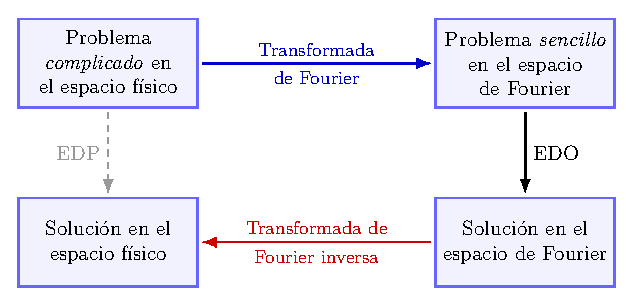
\includegraphics[width = 12cm]{Figuras/Diagrama_Fourier.pdf}
    \caption{Diagrama de uso del método de la transformada de Fourier.}
    \label{fig:Diagrama-Fourier}
\end{figure}

Para hacer más clara esta idea, consideremos el siguiente ejemplo.

\begin{ejemplo}
    Sea la ecuación de difusión del calor dada por
    \begin{equation} \label{eq:Fourier_EDP}
        \frac{1}{\alpha} \frac{\partial u}{\partial t} (x,t) - \frac{\partial^2 u}{\partial x^2}(x,t) = 0 \, , x \in \mathbb{R}, \ t>0 \ ,
    \end{equation}
    con condiciones de contorno dadas por $u(x,0) = \sin(x), \ x \in \mathbb{R}$. Mediante el método de la transformada de Fourier, encuentre la solución al problema.
    
    \textbf{Solución.} Aplicamos la transformada de Fourier \emph{respecto a la coordenada} $x$, de modo que la ecuación \eqref{eq:Fourier_EDP} se transformará en
    \begin{align}
        \mathcal{F}\left\{ \frac{1}{\alpha} \frac{\partial u}{\partial t} - \frac{\partial^2 u}{\partial x^2} \right\}(k, t) & = \mathcal{F}\{0\}(k,t) \nonumber \\
        \frac{1}{\alpha}\mathcal{F}\left\{ \frac{\partial u}{\partial t} \right\}(k, t) - \mathcal{F}\left\{ \frac{\partial^2 u}{\partial x^2} \right\}(k, t) & = 0 \ . \label{eq:Fourier_EDP_transformada}
    \end{align}

    Al hacer uso de la propiedad de la derivada \emph{respecto de la variable de la transformada}, tenemos que
    \begin{equation}
        \mathcal{F}\left\{ \frac{\partial^2 u}{\partial x^2} \right\}(k, t) = (ik)^2 \mathcal{F}\{u\}(k,t) = -k^2 \hat{u}(k,t) \ .
    \end{equation}
    
    Dado que la transformada la hemos calculado \emph{respecto de la posición}, la transformada y la derivada parcial respecto del tiempo conmutan, es decir,
    \begin{align}
        \mathcal{F} \left\{ \frac{\partial u}{\partial t} \right\} & = \frac{1}{\sqrt{2\pi}} \int_{-\infty}^\infty \frac{\partial u}{\partial t} (x,t) e^{-ikx} dx \nonumber \\
        & = \frac{\partial }{\partial t} \left\{ {1}{\sqrt{2\pi}} \int_{-\infty}^\infty u(x,t) e^{-ikx} dx  \right\} \nonumber \\
        & = \frac{\partial \hat{u}}{\partial t}(k,t) \ ,
    \end{align}
    de modo que la ecuación \eqref{eq:Fourier_EDP_transformada} puede reescribirse como
    \begin{equation} \label{eq:EDP_fourier_reducida}
        \frac{1}{\alpha} \frac{\partial \hat{u}}{\partial t}(k,t) + k^2 \hat{u}(k,t) = 0 \ ,
    \end{equation}
    la que puede resolverse como una EDO en la variable $t$, cuya solución particular contiene una constante que, potencialmente, es una función de la variable $k$,
    \begin{equation} \label{eq:solucion_en_fourier}
        \hat{u}(k,t) = A(k) e^{-\alpha k^2 t} \ ,
    \end{equation}
    donde para $t=0$, $\hat{u}(k,0) = A(k)$.

    Aquí, podemos resolver el problema calculando la transformada de Fourier de la condición inicial, que en este caso será
    \begin{equation}
        \mathcal{F}\{u(x,0)\} =  \mathcal{F}\{\sin(x)\} = i \sqrt{\frac{\pi}{2}} [\delta(k+1) - \delta(k-1)] = A(k) \ .
    \end{equation}
    
    Así, la solución a nuestro problema original corresponderá a la transformada de Fourier inversa de la solución \eqref{eq:solucion_en_fourier}, es decir,
    \begin{align}
        u(x,t) & = \frac{1}{\sqrt{2\pi}} \int_{-\infty}^\infty i \sqrt{\frac{\pi}{2}} [\delta(k+1) - \delta(k-1)] e^{-\alpha k^2 t} e^{ikx} dk \nonumber \\
        & = - \frac{1}{2i} \left( e^{-\alpha t} e^{-ix} - e^{-\alpha t} e^{ix} \right) \nonumber \\
        & = e^{-\alpha t} \sin(x) \ . \label{eq:solucion_edp_fourier_final}
    \end{align}
\end{ejemplo}

Un punto de discusión relevante sobre el último ejemplo tiene que ver con el hecho de que no siempre podremos calcular la transformada de Fourier inversa de una forma simple, pues nuestra condición inicial puede no ser tan sencilla. En ese caso, podemos hacer uso de la operación de convolución entre dos funciones, obteniendo una \emph{solución general para la ecuación de difusión del calor}.

\begin{ejemplo}
    \textbf{Solución general a la ecuación de difusión del calor.} Sea la ecuación de difusión del calor dada por
    \begin{equation} \label{eq:Fourier_EDP}
        \frac{1}{\alpha} \frac{\partial u}{\partial t} (x,t) - \frac{\partial^2 u}{\partial x^2}(x,t) = 0 \, , x \in \mathbb{R}, \ t>0 \ ,
    \end{equation}
    con condiciones de contorno general dada por $u(x,0) = u_0$. Mediante el método de la transformada de Fourier, encuentre la solución general al problema.

    \textbf{Solución.} Continuamos desde la ecuación \eqref{eq:solucion_en_fourier}. A partir de esta, tendremos que la transformada inversa tomará la forma
    \begin{equation}
        u(x,t) = \mathcal{F}^{-1} \left\{ \textcolor{red}{\hat{u}_0} \textcolor{blue}{e^{-\alpha k^2 t}} \right\} \ ,
    \end{equation}
    lo que corresponde al producto de dos transformadas de Fourier, la de \textcolor{red}{$\hat{u}_0$} y la de una \textcolor{blue}{gaussiana}, las que pueden ser calculadas gracias a la ecuación \eqref{eq:Fourier-Gaussiana}, con $n=1$ y $\alpha_G = \dfrac{1}{4\alpha t}$.\footnote{Aquí se presenta un abuso de notación que no había considerado anteriormente, ya que en la definición de la gaussiana utilizamos un parámetro $\alpha$, al que he añadido el subíndice $G$ para distinguirlo del coeficiente de difusión de la ecuación del calor.} 
    De este modo, la transformada de Fourier de la gaussiana es
    \begin{equation}
        \mathcal{F}\left\{ e^{-\frac{x^2}{4\alpha t}} \right\} = \sqrt{2\alpha t} e^{-\alpha k^2 t} \ ,
    \end{equation}
    mientras que la transformada inversa toma la forma 
    \begin{equation}
        \mathcal{F}^{-1}\left\{ \textcolor{blue}{e^{-\alpha k^2 t}} \right\} = \frac{e^{-\frac{x^2}{4\alpha t}}}{\sqrt{2\alpha t}}  \ .
    \end{equation}

    Utilizando el teorema de convolución \eqref{Convolucion}, la solución general puede ser obtenida como
    \begin{align}
        u(x,t) & = \frac{1}{\sqrt{2\pi}} \int_{-\infty}^\infty u(v,0) \frac{e^{- \frac{(x-v)^2}{4\alpha t}}}{\sqrt{2\alpha t}} dv \\
        & = \frac{1}{\sqrt{4\pi \alpha t}} \int_{-\infty}^\infty u(v,0) e^{- \frac{(x-v)^2}{4\alpha t}} dv \\
        & = u(x,0) \ast \frac{1}{\sqrt{2\alpha t}}e^{-\frac{x^2}{4\alpha t}} \ .
    \end{align}

    Queda como ejercicio comporbar que para la condición de borde $u(x,0) = \sin(x)$, la solución obtenida por este camino es equivalente a \eqref{eq:solucion_edp_fourier_final}.
\end{ejemplo}